\documentclass[12pt]{article}
\usepackage[margin=1.5cm]{geometry}
\usepackage{parskip}
\usepackage{amsmath}
\usepackage{amssymb}
\usepackage{amsfonts}
\usepackage{enumitem}
\usepackage{graphicx}
\usepackage{stmaryrd}
\graphicspath{ {./images/} }


\begin{document}
\begin{enumerate}[label=(\alph*)]
  \item
    Pairwise sequence alignment algorithms are generally variations of the Needleman-Wunsch algorithm.

    The Needleman-Wunsch algorithm is a dynamic programming algorithm and works by solving the following recurrence relation:

    \[
      F(i,j) = \max\begin{cases}F(i-1, j) + \delta\\F(i, j-1) + \delta\\F(i-1,j-1) + s(x_i, y_j)\end{cases}
    .\] 

    Where $\delta$ is the mismatch penalty, and $s(x_i, y_j)$ is the scoring matrix for matching/mismatching two characters.

    Naively this can be solved by building  an $|x| \times |y|$ matrix, and filling in each cell, and backtracking from the bottom-right cell.

    This takes time and space $O(n^2)$, if $n = \max(|x|, |y|)$.

    However, we can improve both the time and space complexity of this naive algorithm.

    To improve the space complexity, we note that we can compute the matrix column by column, and we only ever need the previous column to compute the next column, which means we can recycle the memory used for columns to allow us to find the maximum alignment score in $O(n)$ space. However, the maximum alignment score alone does not give us an alignment. Instead, we note that if we know the node in the middle column that our path passes through, we can compute our path through a divide and conquer method. We can find the middle node in time proportional to the area of the matrix that we are searching, so finding the initial middle node takes time $O(n^2)$, but finding subsequent middle nodes in the recursive sub-problems will take time $O(\frac{n^2}{2^i})$, so the sum of finding the entire path is still $O(n^2)$. This can still all be done in $O(n)$ space.

    We can also improve the time complexity, although not at the same time as improving the space complexity. This is the Four Russians method, and works by splitting up our matrix into blocks of size $t = \frac{\log n}{4}$. We can precompute the alignment scores for each block in a lookup table, and then search this lookup table to find a path through our blocks (we store extra information in our lookup table to handle movement not in block corners). The lookup table size will be of size $n^{\frac{3}{2}}$, and thus the time complexity will be $O(\frac{n^2}{\log n})$.

  \item
    Clustering is the process of taking a set of $n$-dimensional points, and dividing them into a number of clusters, ideally such that we obey the good clustering principle, which is that elements within the same cluster are close to each other than elements in different clusters.

    Hard clustering is when each point is assigned exactly one cluster, and soft clustering is a variation where each point is assigned a vector (with elements summing to 1), where each element in the vector corresponds to the `responsibility' that that cluster has over that point.

    An example of hard clustering is the $k$-means algorithm, where we create $k$ arbitrary `center ppoints', and cluster each point based on its closest center, and then move the center point of each cluster to the average of each of its point's positions. We then iterate this process until convergence.

    An example of soft clustering is using expectation maximisation. Again, we randomly choose an arbitrary $k$ centers, and compute responsibilities for each point in our dataset. Then, we use these responsibilities to re-estimate our $k$ centers. We change the stiffness of our soft clustering by changing how we calculate the responsibilities for each center.

  \item
    We choose $k=3$, giving the following $k$-mers:

\begin{verbatim}
TAC
ACC
CCT
CTT
TTC
TCA
CAG
AGC
GCG
CGC
GCC
CCT
CTT
TTC
\end{verbatim}

Giving us the following De Bruijn graph:

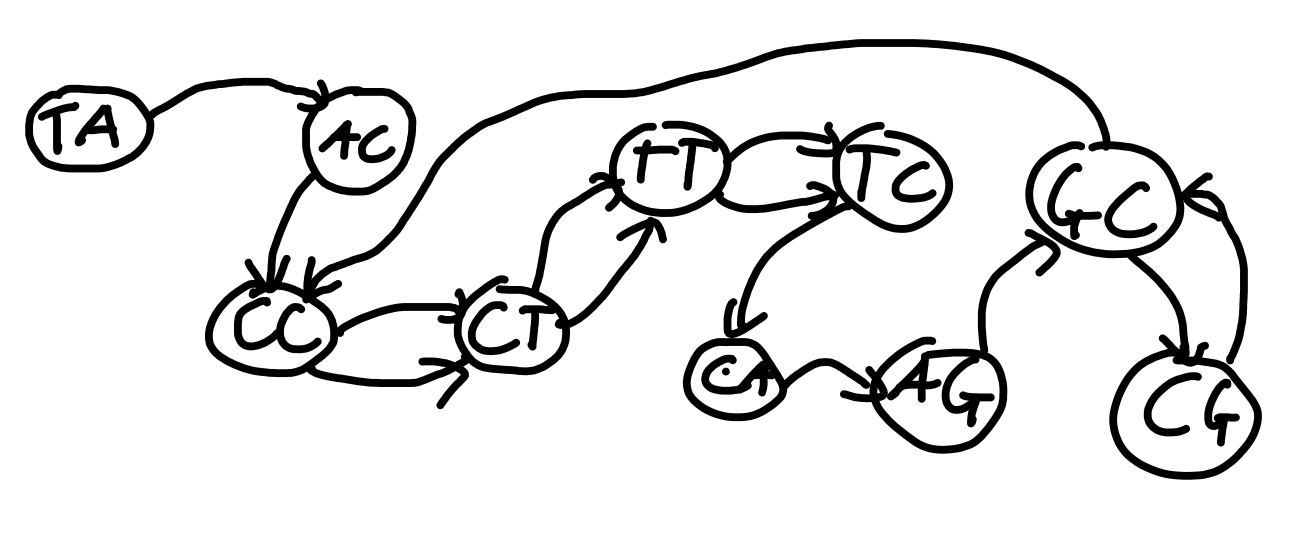
\includegraphics[scale=0.3]{debruijn}

Increasing $k$ makes the number of edges lower, but might make the number of nodes larger, since we are less likely to have duplicates.

In genome sequencing, we can use De Bruijn graphs to sequence a genome by taking a number of reads of our genome, and converting all of them into $k$-mers. Then, we use all of these $k$-mers to construct a De Bruijn graph, and the problem of genome sequencing then becomes a problem of finding an Eulerian path through the graph, which is solvable in $O(|E|)$ time, which is the number of $k$-mers we have.


        
\end{enumerate}
\end{document}
